\chapter{Umsetzung}
In diesem Abschnitt wird die technische Realisierung des Projekts dargestellt. 
Zunächst wird die Systemarchitektur beschrieben, anschließend werden die 
eingesetzten Technologien erläutert. Im Anschluss folgt eine detaillierte 
Darstellung der implementierten Funktionen zum Import, zur Bearbeitung, 
Suche, Löschung und zum Export von Bib\TeX{}-Daten.

\section{Systemarchitektur}
Das entwickelte Assistenzsystem für wissenschaftliches Arbeiten basiert auf einer klar strukturierten 3-Schichten-Architektur. 
Es besteht aus einem Frontend zur Benutzerinteraktion, einem Backend zur Verarbeitung der Anfragen sowie einer lokalen Datenbank 
zur temporären Datenhaltung.\\

\noindent Das Frontend wurde mit React, JavaScript und CSS implementiert, um eine erfolgreiche Benutzerinteraktion zu ermöglichen. 
Über das Frontend können Professor:innen sowie andere Personen mit wissenschaftlichen Publikationen BibTeX-Dateien importieren, 
deren Einträge bearbeiten oder löschen und anschließend als XML-Datei exportieren, um sie in OPUS zu importieren. Das Backend 
wurde mit Node.js und Express realisiert und stellt über definierte Endpoints die Schnittstelle zwischen Frontend und Datenbank 
bereit. Es übernimmt die Verarbeitung der Import- und Exportvorgänge sowie die Datenpersistenz. Die lokale Datenspeicherung 
erfolgt im Local Storage des Systems, wodurch keine externe Datenbankverbindung notwendig ist. Dies vereinfacht die Architektur, 
ermöglicht aber dennoch das Zwischenspeichern von Daten zwischen verschiedenen Arbeitsschritten innerhalb einer Sitzung.

\begin{figure}[h]
    \centering
    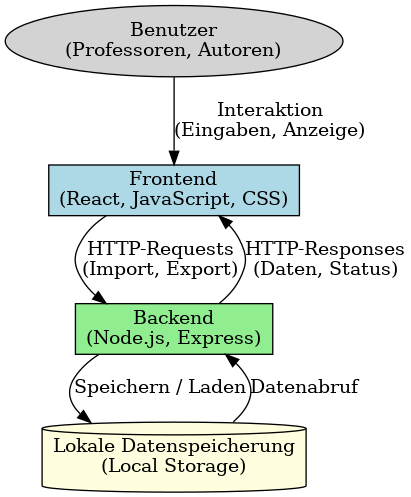
\includegraphics[width=0.5\textwidth]{Graphics/systemarchitektur_diagramm.png}
    \caption{Systemarchitektur des entwickelten Assistenzsystems}
    \label{fig:systemarchitektur}
\end{figure}

\section{Technologie-Stack}
Das Assistenzsystem wurde mit moderne und effektive Technologie Stack
entwickelt, der eine einfache Wartung ermöglicht. Der Stack umfasst sowohl
Frontend und Backend Technologien sowie die lokalen Datenspeicherung.

\subsection{Frontend}
Für die Benutzeroberfläche wurde das React-Framework in Kombination mit JavaScript eingesetzt. 
React ermöglicht eine komponentenbasierte Entwicklung. Dadurch sind einzelne Funktionseinheiten 
wie Importformulare, Bearbeitungsansichten und Exportfunktionen klar voneinander getrennt und 
wiederverwendbar. Um eine ansprechende und benutzerfreundliche Oberfläche zu gewährleisten, 
wurden die Gestaltung und das Layout mit CSS umgesetzt.

\subsection{Backend}
Die serverseitige Logik basiert auf Node.js mit dem Express-Framework. Durch die Verwendung von 
Node.js wird eine ereignisgesteuerte und asynchrone Verarbeitung ermöglicht, wodurch die Verarbeitung 
von Benutzeraktionen beschleunigt werden kann. Express bietet eine klare Struktur für die Definition 
von Endpoints, über die das Frontend mit dem Backend kommuniziert. Die vorliegende Arbeit befasst 
sich mit REST-Endpoints, die insbesondere für die Steuerung von Import- und Exportprozessen sowie für 
den Zugriff auf die lokale Datenspeicherung genutzt werden.

\subsection{Datenhaltung}
Für die Datenspeicherung wird der Local Storage des Browsers verwendet. Dieser ermöglicht eine einfache, 
eingeschränkt persistente Ablage der importierten BibTeX-Dateien, die auch nach dem Schließen des Browsers 
erhalten bleibt. Da die Daten lediglich als temporäre Zwischenablage dienen und anschließend im OPUS-Format 
exportiert werden, ist der Einsatz einer vollwertigen Datenbank nicht erforderlich. Diese Entscheidung 
reduziert die Systemkomplexität und genügt den Anforderungen des Systems.


\section{Implementierung der Features}

\subsection{Parsen und API-Kommunikation}
Zu Beginn wurde ein Parser-Service implementiert, der eine hochgeladene \texttt{.bib}-Datei einliest 
und deren Inhalte in ein strukturiertes JSON-Format umwandelt. Dies ermöglicht eine einfache Weiterverarbeitung 
der Literaturdaten im Frontend. Dabei wurden Bibliotheken genutzt, um die einzelnen Felder wie Titel, Autoren, Jahr
und Publikationsart korrekt zu extrahieren.\\

\noindent Für die Kommunikation zwischen Backend und Frontend wurden mehrere REST-API-Endpunkte erstellt.
Diese liefern die geparsten Daten im JSON-Format, nehmen Änderungen vom Frontend entgegen und
stellen Funktionen zum Speichern und Löschen bereit. Die Endpunkte wurden so gestaltet, dass sie sowohl
einzelne Einträge als auch komplette Datensätze verarbeiten können.

\subsection{Importieren, Bearbeiten und Trennen der Einträge}
Im Frontend wurde ein Button \glqq Importieren\grqq{} implementiert, der es dem Benutzer ermöglicht,
eine lokale \texttt{.bib}-Datei auszuwählen. Nach der Auswahl wird die Datei an das Backend gesendet, 
dort geparst und die verarbeiteten Daten werden im Frontend angezeigt.

\begin{figure}[h]
    \centering
    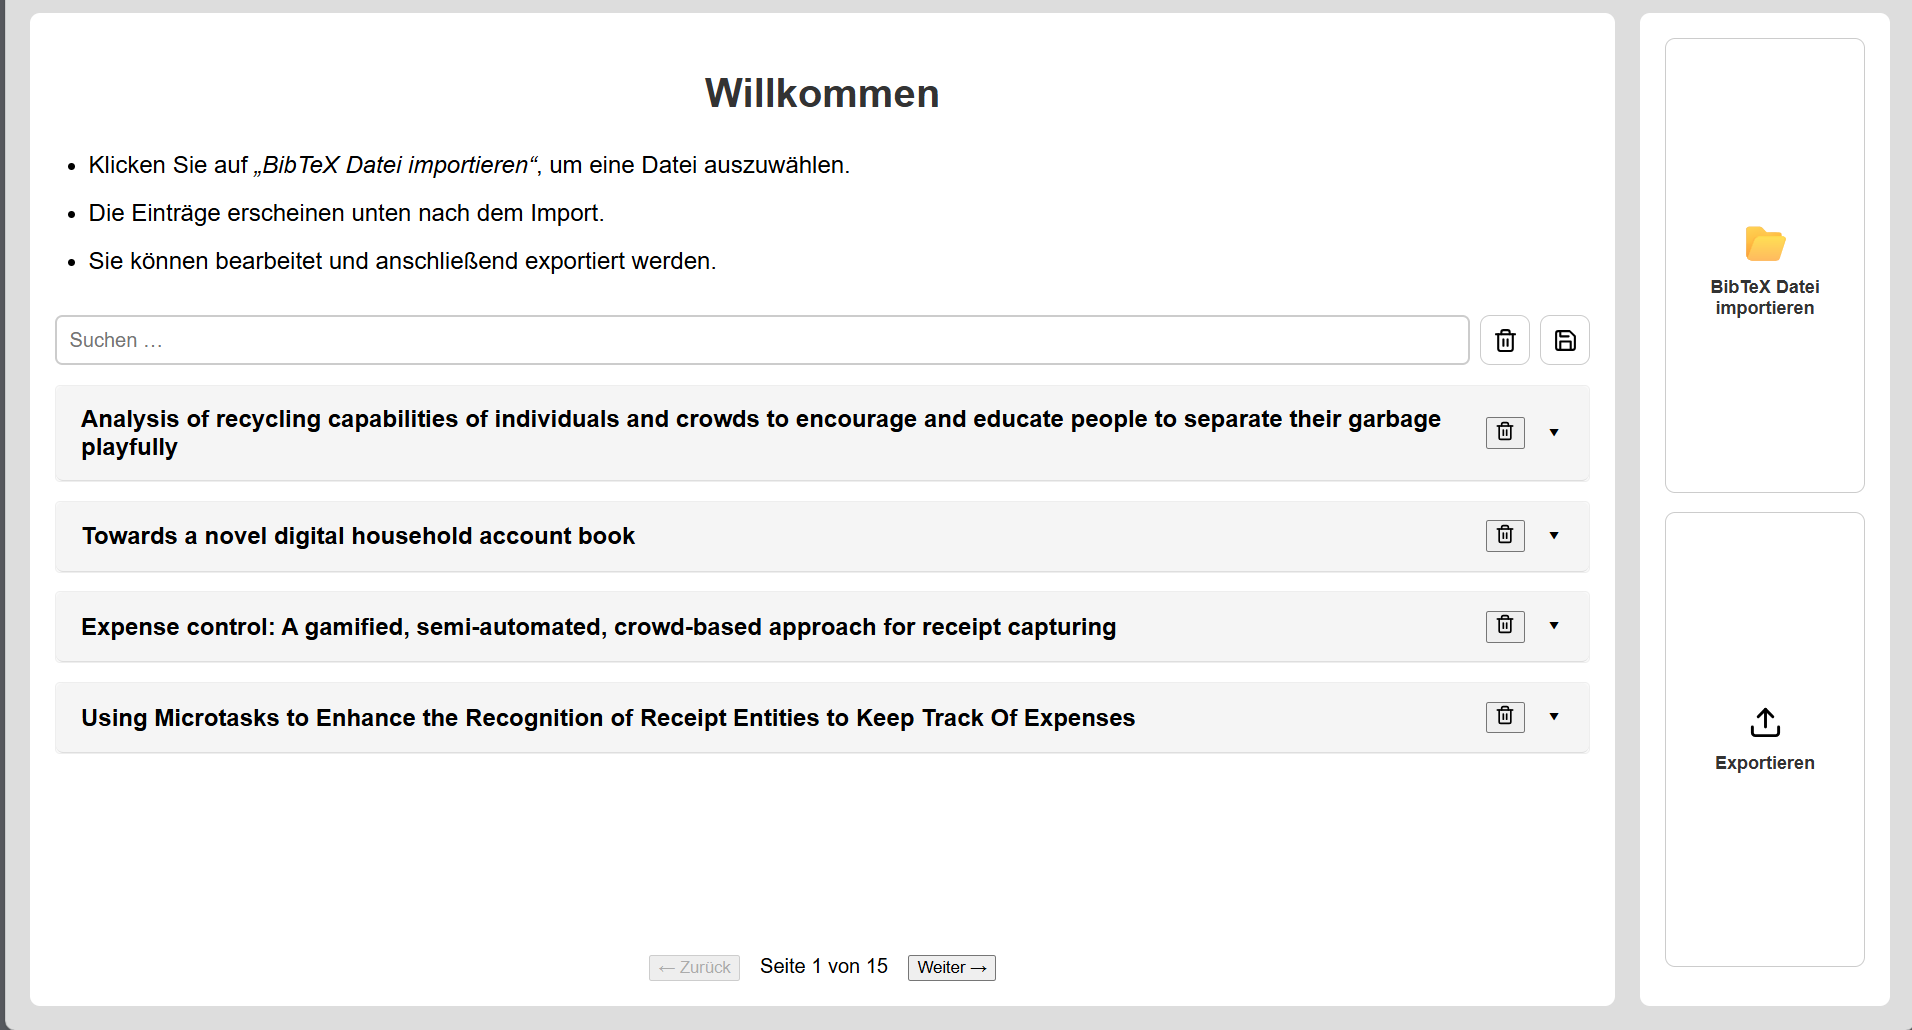
\includegraphics[width=0.8\textwidth]{Graphics/front.png}
    \caption{Benutzeroberfläche des Import-Buttons und Trennen der Einträge}
    \label{fig:importieren}
\end{figure}

\noindent Jeder Eintrag kann direkt in der Oberfläche bearbeitet werden. Änderungen an Feldern wie Titel,
Autoren oder Jahr werden sofort in der aktuellen Ansicht übernommen und können später gespeichert werden.
Eine spezielle Logik trennt die Autorenangaben aus der \texttt{.bib}-Datei in einzelne Felder.
Dies erlaubt eine saubere Darstellung und erleichtert die Bearbeitung einzelner Namen.

\begin{figure}[h]
    \centering
    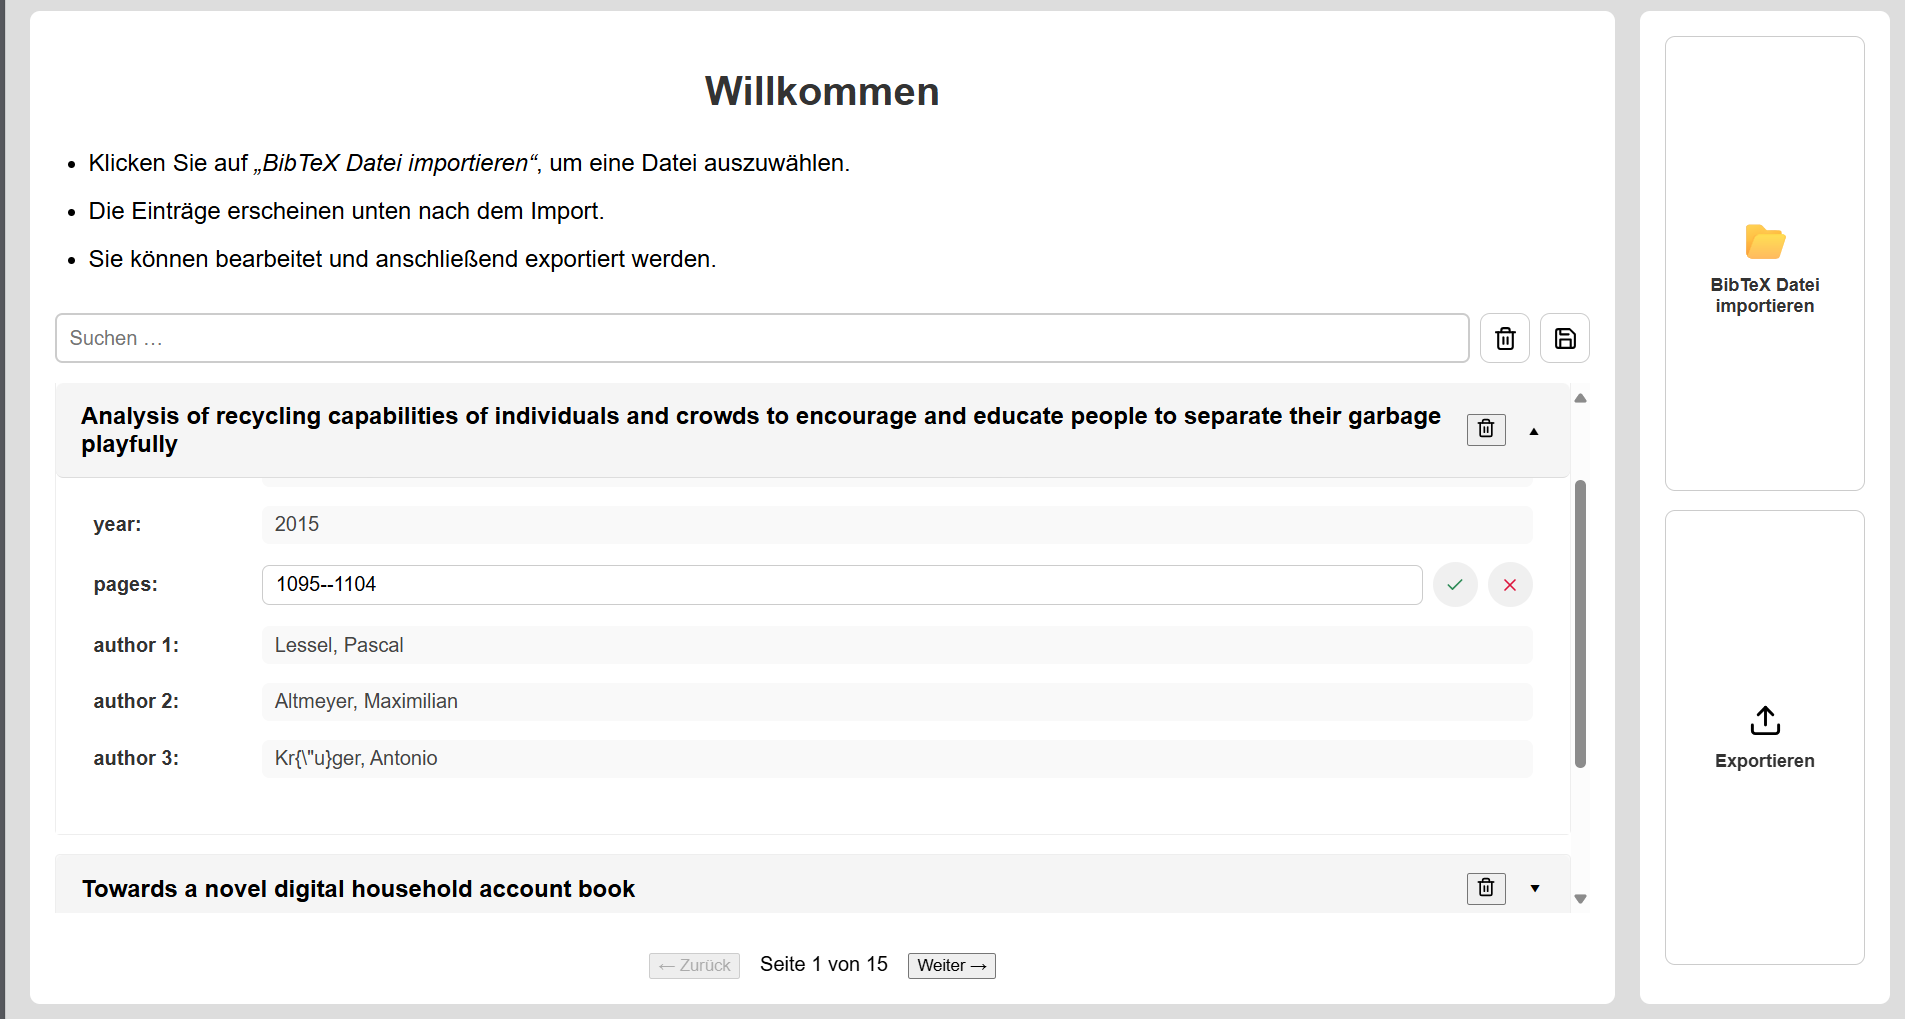
\includegraphics[width=0.8\textwidth]{Graphics/frontend.png}
    \caption{Bearbeitung eines Literatur-Eintrags}
    \label{fig:bearbeiten}
\end{figure}

\subsection{Anzeige und Navigation der Einträge}
Um die Übersichtlichkeit zu erhöhen, werden die einzelnen Literatur-Einträge in einer aufklappbaren
Struktur dargestellt. So kann der Benutzer gezielt die Details eines Eintrags einsehen oder ausblenden.\\

\noindent Um die Navigation bei vielen Einträgen zu vereinfachen, wurde eine Paginierung implementiert.
Diese teilt die Liste der Einträge in mehrere Seiten auf und reduziert so die Ladezeit und die visuelle Überlastung.

\subsection{Such- und Löschfunktionen}
Eine Suchkomponente ermöglicht das Filtern von Einträgen anhand von Schlagwörtern.
Dies erleichtert das Auffinden bestimmter Publikationen in großen Datenbeständen.

\noindent Mit dem Button \glqq Alle löschen\grqq{} können sämtliche Einträge in der aktuellen Ansicht entfernt werden.
Diese Funktion ist besonders nützlich, wenn ein neuer Datensatz importiert werden soll.

\subsection{Speicherung und Export der Daten}
Über den Local Storage des Browsers werden Änderungen lokal gespeichert,
sodass diese auch nach einem Neuladen der Seite erhalten bleiben.
Diese Funktion dient als Zwischenspeicher, bevor die Daten endgültig exportiert oder gespeichert werden.
Der Button \glqq Speichern\grqq{} ermöglicht es, alle vorgenommenen Änderungen dauerhaft zu sichern.
Dabei werden die aktuellen Daten aus dem Local Storage übernommen und entweder im Backend oder als Exportdatei gespeichert.\\

\noindent Zum Schluss  bietet der Button \glqq Exportieren\grqq{} die Möglichkeit,
alle gespeicherten Daten in eine XML-Datei umzuwandeln und herunterzuladen.Diese Datei kann später in OPUS importiert werden .
